%%%========================== %%%
%%%  Set Beamer as class        
%%%==========================%%%
%%
%% Beamer
\documentclass{beamer}
\setbeamercovered{transparent}

%%%========================== %%%
%%%  Set theme        
%%%==========================%%%
%%
%% Warsaw
\usetheme{Warsaw}

%%%========================== %%%
%%%  German Umlauts                            
%%%==========================%%%
%%
%% For Mac OS X
%% \usepackage[applemac]{inputenc}
%% For PC Windows
%% \usepackage[ansinew]{inputenc}
%%
%% For PC Linux 
%% \usepackage[latin1]{inputenc}
%%
%% For UTF-8
\usepackage[utf8]{inputenc}

%%%========================== %%%
%%%  German hyphenation              
%%%==========================%%%
%%
\usepackage{ngerman}

%%%========================== %%%
%%%  Quotes
%%%  \enquote{}       
%%%==========================%%%
%%
\usepackage[babel,german=quotes]{csquotes}

%%%========================== %%%
%%%  Tikz   
%%%==========================%%%
%%
\usepackage{xcolor}
\usepackage{tikz,pgffor}
\usetikzlibrary{shadows}
\tikzset{
	MyPersp/.style={scale=1.8,x={(-0.8cm,-0.4cm)},y={(0.8cm,-0.4cm)},
    z={(0cm,1cm)}},
%  MyPersp/.style={scale=1.5,x={(0cm,0cm)},y={(1cm,0cm)},
%    z={(0cm,1cm)}}, % uncomment the two lines to get a lateral view
	MyPoints/.style={fill=white,draw=black,thick}
		}

% #1 number of teeths
% #2 radius blanket intern
% #3 radius blanket extern
% #4 angle from start to end of the first arc
% #5 angle to decale the second arc from the first 
% #6 radius dna intern
% #7 radius dna extern
% #8 xshift
\newcommand{\gear}[8]{%
  \foreach \i in {1,...,#1} {%
    [rotate=(\i-1)*360/#1]  (0:#2)  arc (0:#4:#2) {[rounded corners=2pt]
     -- (#4+#5:#3)  arc (#4+#5:360/#1-#5:#3)} --  (360/#1:#2)
  }%
  (0,0) circle[radius=#6]
  (0,0) circle[radius=#7];
\draw[thick,xshift=#8]
\foreach \i in {1,2,...,36} {%
  [rotate=(\i-1)*10]  (0.0,#6) -- (0.0,#7)
};
}  

\usepackage{hyperref}


%%%========================== %%%
%%%  Settings for the startpage              
%%%==========================%%%
%%
\title{Introducing: \enquote{The Machine} (DRAFT)}
\author{\texorpdfstring{\ Jürgen Scholz \ \newline\url{j.scholz@machinecoin.org}}{Author}}
\institute{The Machine - A complete self-contained cryptographic ecosphere driven by nothing but the Machinecoin cryptocurrency.}
\date{2014/06/02}

%%%========================== %%%
%%%  Document Start                                
%%%==========================%%%
%%
\begin{document}
\frame{\titlepage}

\frame
{
\tableofcontents
}

\section{Introduction}

\frame
{   
In November 2008, a paper titled ``Bitcoin: A Peer-to-Peer Electronic Cash System'' was posted on The Cryptography Mailing List at metzdowd.com. It was written by either a person or group with the pseudonymous ``Satoshi Nakamoto''. In this paper methods of using a peer-to-peer network to generate a system for electronic transactions without relying on trust were described in detail.
\newline
\newline
\visible<2->{\texttt{``A purely peer-to-peer version of electronic cash would allow online payments to be sent directly from one party to another without going through a financial institution.''}
  \vskip5mm
  \hspace*\fill{\small--- Satoshi Nakamoto, Bitcoin: A Peer-to-Peer Electronic Cash System\footnote{http://bitcoin.org/bitcoin.pdf}}}
}

\frame
{   
In January 2009, these methods came into existence through the release of the first open source Bitcoin client and the issuance of the first bitcoins, with Satoshi Nakamoto, mining the first block of bitcoins, which at this time had a reward of 50 bitcoins. 
\newline
\newline
\visible<2->{In the beginning the values of the first bitcoin transactions were negotiated by individuals on the bitcointalk forums with for example one notable transaction involving a pizza for 10,000 bitcoins\footnote{https://bitcointalk.org/index.php?topic=137.0}.}
\newline
\newline
\visible<3->{These transactions provided a good evidence that it is not just in theory but also in practice possible to have a purely peer-to-peer electronic cash without the need to go through a financial institution.}
}

\frame
{   
Since then a lot of alternative cryptocurrencies have been created. All or most of them are working on the same basis just as Bitcoin does but with slightly different algorithms for special tasks.  
\newline
\newline
\visible<2->{So in general nothing seems to may have changed despite one thing: the major of the cryptoscene has turned cryptocurrencies away from being electronic cash into something that could be better described as classical currency slaves.}
\newline
\newline
\visible<3->{This means that their ``values''\footnote{http://gitju.github.io/Machinecoin.org/wp-content/uploads/2014/04/value.pdf} are rather determined by exchange rates than by real available products or services which a (crypto)currency originally is made for and therefore the cryptoscene has lost the path.}
}

\frame
{
So lets go back to basic and have a look at the primary function of any given (crypto)currency:
\newline
\setbeamercovered{transparent}
\begin{enumerate} 
\item<2-> A (crypto)currency is a medium that makes exchanges of products and/or services between two parties (buyer/seller) possible ...
\item<3-> ... even if the one who is the buyer has got no product and/or service available ...
\item<4-> ... that the seller would like to have and the buyer would like to give in exchange for it
\end{enumerate} 
\ 
\newline
\visible<5->{To focus on this we have decided to model a complete self-contained cryptographic ecosphere driven by nothing but the Machinecoin cryptocurrency.}
}

\frame
{
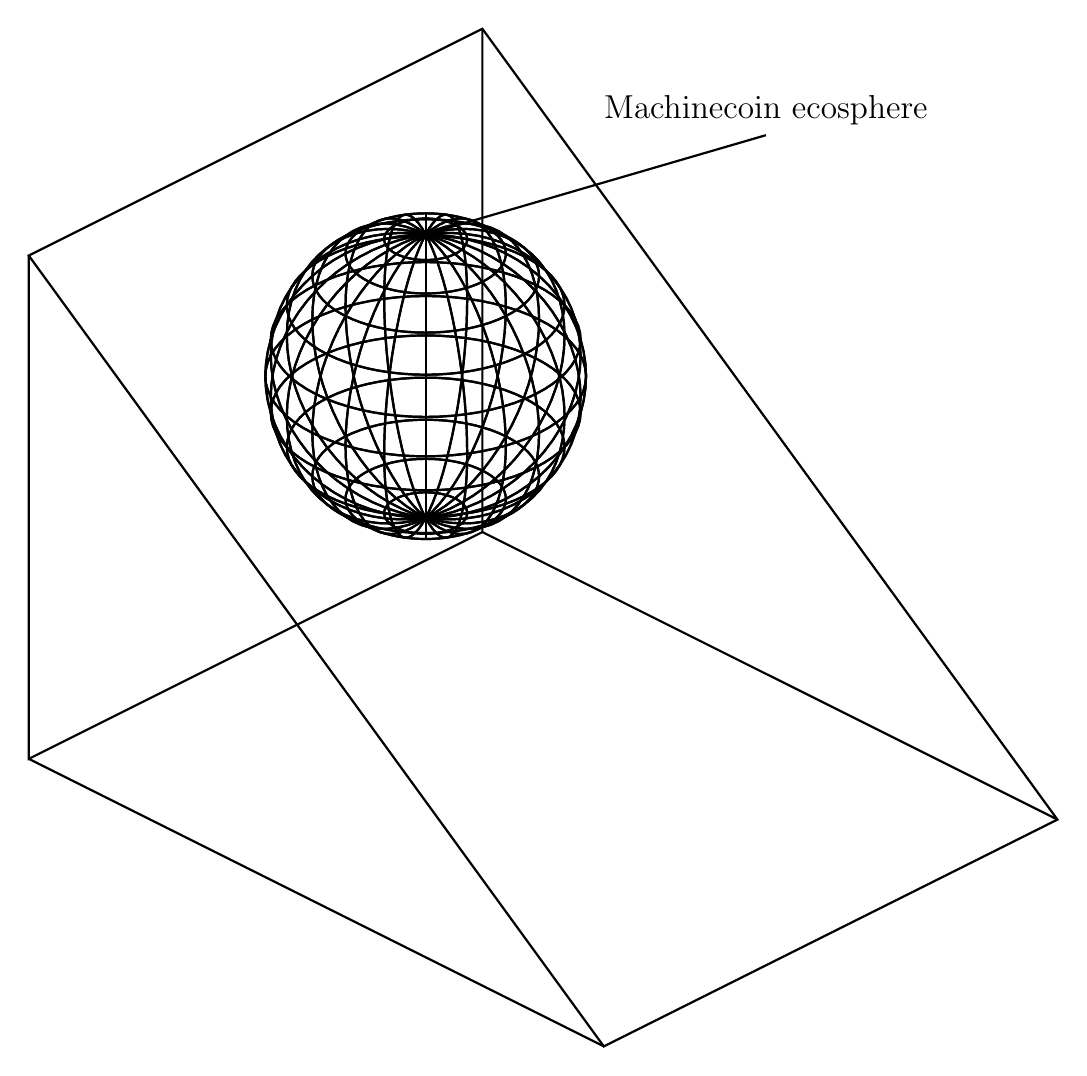
\begin{tikzpicture}[MyPersp,font=\large]
	\def\h{2.5}% Heigth of the ellipse center 
	\def\a{35}% Angle of the section plane with the horizontal
	\def\aa{35}% Angle that defines position of generatrix PA--PB
	\pgfmathparse{\h/tan(\a)}
  	\let\b\pgfmathresult
	\pgfmathparse{sqrt(1/cos(\a)/cos(\a)-1)}
  	\let\c\pgfmathresult %Center Focus distance of the section ellipse.
	\pgfmathparse{\c/sin(\a)}
  	\let\p\pgfmathresult % Position of Dandelin spheres centers
     					% on the Oz axis (\h +/- \p)
	\coordinate (A) at (2,\b,0);
	\coordinate (B) at (-2,\b,0);
	\coordinate (C) at (-2,-1.5,{(1.5+\b)*tan(\a)});
	\coordinate (D) at (2,-1.5,{(1.5+\b)*tan(\a)});
	\coordinate (E) at (2,-1.5,0);
	\coordinate (F) at (-2,-1.5,0);
	\coordinate (CLS) at (0,0,{\h-\p});
	\coordinate (CUS) at (0,0,{\h+\p});
	\coordinate (FA) at (0,{\c*cos(\a)},{-\c*sin(\a)+\h});% Focii
	\coordinate (FB) at (0,{-\c*cos(\a)},{\c*sin(\a)+\h});
	\coordinate (SA) at (0,1,{-tan(\a)+\h}); % Vertices of the
                                           % great axes of the ellipse
	\coordinate (SB) at (0,-1,{tan(\a)+\h});
	\coordinate (PA) at ({sin(\aa},{cos(\aa)},{\h+\p});
	\coordinate (PB) at ({sin(\aa},{cos(\aa)},{\h-\p});
	\coordinate (P) at ({sin(\aa)},{cos(\aa)},{-tan(\a)*cos(\aa)+\h});
     % Point on the ellipse on generatrix PA--PB

	\draw[thick] (A)--(B)--(C)--(D)--cycle;
	\draw[thick] (D)--(E)--(F)--(C);
	\draw[thick] (A)--(E) (B)--(F);


	\foreach \i in {0,0}{%Spheres!
		\foreach \t in {0,15,...,165}% meridians
			{\draw[thick,-] ({cos(\t)},{sin(\t)},\h+\i*\p)
				\foreach \rho in {5,10,...,360}
					{--({cos(\t)*cos(\rho)},{sin(\t)*cos(\rho)},
          {sin(\rho)+\h+\i*\p})}--cycle;
			}
		\foreach \t in {-75,-60,...,75}% parallels
			{\draw[thick,-] ({cos(\t)},0,{sin(\t)+\h+\i*\p})
				\foreach \rho in {5,10,...,360}
					{--({cos(\t)*cos(\rho)},{cos(\t)*sin(\rho)},
          {sin(\t)+\h+\i*\p})}--cycle;
			}
		}

    \draw[thick,-] (17.5,17.5,17.5) -- (17,20,19) node[right,above]{Machinecoin ecosphere};
\end{tikzpicture}
}

\frame
{
\begin{definition}[Machinecoin ecosphere]
The Machinecoin ecosphere is a complete self-contained cryptographic ecosphere driven by nothing but the Machinecoin cryptocurrency.
\end{definition}
\  
\newline
%\visible<2->{It consists of for example all products and services that are available in exchange to Machinecoin. Furthermore: all direct participants of transactions l%ike buyer and seller but also indirect participants like miner and developer are part of the entire Machinecoin ecosphere.} 
%\newline
%\newline
\visible<2->{To better understand what this means someone could imagine to put all the people that are involved into the Machinecoin cryptocurrency together into a country where just the Machinecoin would exist as a currency.}
\newline
\newline
\visible<3->{All inhapitants of that country with all their activities would then define the Machinecoin ecosphere.}
}

\frame
{
The Machinecoin ecosphere consists of the following participants
\begin{enumerate}
\item<2-> Machinists. All participants of the Machinecoin ecosphere are Machinists. For the Machinecoin ecosphere they are like atoms.
\item<3-> Blanks. They are made of 1 or more Machinists that contain the entire Machinecoin source code. Basically any Blank owns everything that would be necessary to recreate the entire Machinecoin ecosphere from scratch. For the Machinecoin ecosphere they are like constructs made of stem cells.
\item<4-> Gears. All Blanks that offer any kind of special Machinecoin infrastructure are called to be Gears. For the Machinecoin ecosphere they are like constructs made of differentiated cells.  
\end{enumerate}
\ 
\newline
\visible<5->{The complex interacting between all those participants forms \texttt{The Machine}.}
}

\frame
{
%\begin{figure}
\centering
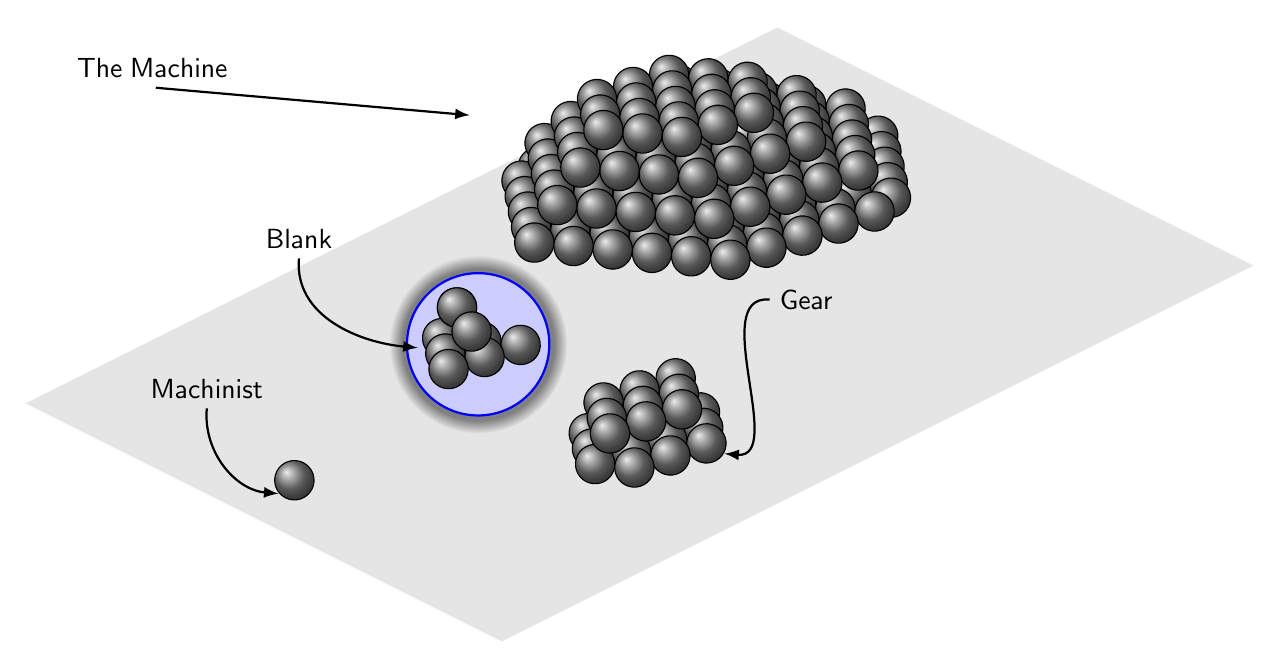
\begin{tikzpicture}
%\draw[help lines] (0,0) grid (10,10); %used just for visualising the positions of objects during construction

\begin{scope}[yshift=-180,yslant=0.5,xslant=-1]
    %the rectangular surface onto which the clusters are located
    \filldraw[black!10,very thick] (0.5,1) rectangle (10,7);
    %circle circumventing the smallest cluster 
    \node[circle,circular glow,fill=blue!20,draw=blue,thick]
    at (4.1,4.9) {\phantom{perimetro}};
\end{scope}

%atom clusters are rotated for a better visualisation
\begin{scope}[rotate around = {-5:(0,0,0)}]
    %text describing the objects in the picture
    \draw[-latex,thick] (-5,1) node[above,text width=2cm] 
        {$\mathsf{The\; Machine}$} to [out=0,in=180] (-1,1);
    \draw[-latex,thick](3,-1)node[right]
        {$\mathsf{Gear}$} to[out=180,in=0] (2.6,-3);
    \draw[-latex,thick](-3,-1)node[above]
        {$\mathsf{Blank}$} to[out=-90,in=180] (-1.4,-2);

    %now we start with the clusters (maybe this code could be improved by a tikz expert)
    %the layers are built starting from the very lowest one

    %largest cluster
    %first row
    \foreach \x  in {1.5,2,2.5,3,3.5,4}%
        \shadedraw [ball color= gray] (\x,1,-0.5) circle (0.25cm);
    \foreach \x  in {1.25,1.75,2.25,2.75,3.25,3.75,4.25}%
        \shadedraw [ball color= gray] (\x,1,0) circle (0.25cm);
    \foreach \x  in {1,1.5,2,2.5,3,3.5,4,4.5}%
        \shadedraw [ball color= gray] (\x,1,0.5) circle (0.25cm);
    \foreach \x  in {0.75,1.25,1.75,2.25,2.75,3.25,3.75,4.25,4.75}%
        \shadedraw [ball color= gray] (\x,1,1) circle (0.25cm);
    \foreach \x  in {0.5,1,1.5,2,2.5,3,3.5,4,4.5,5}%
        \shadedraw [ball color= gray] (\x,1,1.5) circle (0.25cm);
    \foreach \x  in {0.5,1,1.5,2,2.5,3,3.5,4,4.5,5}
        \shadedraw [ball color=gray] (\x,1,2) circle (0.25cm);
    \foreach \x  in {0.75,1.25,1.75,2.25,2.75,3.25,3.75,4.25,4.75}%
        \shadedraw [ball color= gray] (\x,1,2.5) circle (0.25cm);
    \foreach \x  in {1,1.5,2,2.5,3,3.5,4,4.5}%
        \shadedraw [ball color= gray] (\x,1,3) circle (0.25cm);
    \foreach \x  in {1.25,1.75,2.25,2.75,3.25,3.75,4.25}%
        \shadedraw [ball color= gray] (\x,1,3.5) circle (0.25cm);
    \foreach \x  in {1.5,2,2.5,3,3.5,4}%
        \shadedraw [ball color= gray] (\x,1,4) circle (0.25cm);
    %second row 
    \foreach \x  in {1.75,2.25,2.75,3.25,3.75}
        \shadedraw [ball color=gray] (\x,1.5,0) circle (0.25cm);
    \foreach \x  in {1.5,2,2.5,3,3.5,4}
        \shadedraw [ball color=gray] (\x,1.5,0.5) circle (0.25cm);
    \foreach \x  in {1.25,1.75,2.25,2.75,3.25,3.75,4.25}
        \shadedraw [ball color=gray] (\x,1.5,1) circle (0.25cm);
    \foreach \x  in {1,1.5,2,2.5,3,3.5,4,4.5}
        \shadedraw [ball color=gray] (\x,1.5,1.5) circle (0.25cm);
    \foreach \x  in {0.75,1.25,1.75,2.25,2.75,3.25,3.75,4.25,4.75}
        \shadedraw [ball color=gray] (\x,1.5,2) circle (0.25cm);
    \foreach \x  in {1,1.5,2,2.5,3,3.5,4,4.5}
        \shadedraw [ball color=gray] (\x,1.5,2.5) circle (0.25cm);
    \foreach \x  in {1.25,1.75,2.25,2.75,3.25,3.75,4.25}
        \shadedraw [ball color=gray] (\x,1.5,3) circle (0.25cm);
    \foreach \x  in {1.5,2,2.5,3,3.5,4}
        \shadedraw [ball color=gray] (\x,1.5,3.5) circle (0.25cm);
    \foreach \x  in {1.75,2.25,2.75,3.25,3.75}
        \shadedraw [ball color=gray] (\x,1.5,4) circle (0.25cm);
    %third row 
    \foreach \x  in {2,2.5,3,3.5}
        \shadedraw [ball color=gray] (\x,2,1) circle (0.25cm);
    \foreach \x  in {1.75,2.25,2.75,3.25,3.75}
        \shadedraw [ball color=gray] (\x,2,1.5) circle (0.25cm);
    \foreach \x  in {1.5,2,2.5,3,3.5,4}
        \shadedraw [ball color=gray] (\x,2,2) circle (0.25cm);
    \foreach \x  in {1.25,1.75,2.25,2.75,3.5,3.75,4.25}
        \shadedraw [ball color=gray] (\x,2,2.5) circle (0.25cm);
    \foreach \x  in {1.5,2,2.5,3,3.5,4}
        \shadedraw [ball color=gray] (\x,2,3) circle (0.25cm);
    \foreach \x  in {1.75,2.25,2.75,3.25,3.75}
        \shadedraw [ball color=gray] (\x,2,3.5) circle (0.25cm);
    \foreach \x  in {2,2.5,3,3.5}
        \shadedraw [ball color=gray] (\x,2,4) circle (0.25cm);
    %fourth row
    \foreach \x  in {2.25,2.75,3.25}
        \shadedraw [ball color=gray] (\x,2.5,2) circle (0.25cm);
    \foreach \x  in {2,2.5,3,3.5}
        \shadedraw [ball color=gray] (\x,2.5,2.5) circle (0.25cm);
    \foreach \x  in {1.75,2.25,2.75,3.25,3.75}
        \shadedraw [ball color=gray] (\x,2.5,3) circle (0.25cm);
    \foreach \x  in {2,2.5,3,3.5}
        \shadedraw [ball color=gray] (\x,2.5,3.5) circle (0.25cm);
    \foreach \x  in {2.25,2.75,3.25}
        \shadedraw [ball color=gray] (\x,2.5,4) circle (0.25cm);

    %medium cluster
    %first row
    \foreach \x  in {6.75,7.25}
        \shadedraw [ball color=gray] (\x,2.5,13) circle (0.25cm);
    \foreach \x  in {6.5,7,7.5}
        \shadedraw [ball color=gray] (\x,2.5,13.5) circle (0.25cm);
    \foreach \x  in {6.25,6.75,7.25,7.75}
        \shadedraw [ball color=gray] (\x,2.5,14) circle (0.25cm);
    \foreach \x  in {6.5,7,7.5}
        \shadedraw [ball color=gray] (\x,2.5,14.5) circle (0.25cm);
    \foreach \x  in {6.75,7.25}
        \shadedraw [ball color=gray] (\x,2.5,15) circle (0.25);

    %second row
    \foreach \x  in {7} %this foreach is used to be general, but it makes no sense if we put just one sphere!
        \shadedraw [ball color=gray] (\x,3,13.25) circle (0.25cm);
    \foreach \x  in {6.75,7.25}
        \shadedraw [ball color=gray] (\x,3,13.75) circle (0.25cm);
    \foreach \x  in {6.5,7,7.5}
        \shadedraw [ball color=gray] (\x,3,14.25) circle (0.25cm);
    \foreach \x  in {6.75,7.25}
        \shadedraw [ball color=gray] (\x,3,14.75) circle (0.25cm);
    \foreach \x  in {7}
        \shadedraw [ball color=gray] (\x,3,15.25) circle (0.25);

    %smallest cluster of atoms

    \foreach \x in {2.75,3.25,3.75}
        \shadedraw [ball color = gray] (\x,2,10) circle (0.25);
    \foreach \x in {3,3.5}
        \shadedraw [ball color=gray] (\x,2,10.5) circle (0.25);
    \shadedraw [ball color = gray] (3.25,2,11) circle (0.25);
    \foreach \x in {3,3.5}
        \shadedraw [ball color = gray] (3,2.5,10.25) circle (0.25);
    \shadedraw [ball color = gray] (3.5,2.5,11) circle (0.25);

    \shadedraw [ball color=gray] (2,1,12.5) circle(0.25);
    \draw[-latex,thick](-4,-3)node[above]
        {$\mathsf{Machinist}$} to[out=-90,in=180] (-3,-4);
\end{scope}
\end{tikzpicture}
%\end{figure}
}

%\frame
%{
%\begin{figure}[htbp]
%\includegraphics[width=80mm,height=61mm]{glas.jpg}
%\end{figure}
%}

%\begin{frame}{Title}{Subtitle}
%   \begin{columns}
%        \begin{column}{.5\textwidth}
%            Your longish paragraph text here, where you describe stuff and so on
%        \end{column}
%        \begin{column}{.5\textwidth}\raggedleft
%            \includegraphics[width=4cm,height=4cm]{glas.jpg}
%        \end{column}
%    \end{columns}
% \end{frame}

\section{Basics}
%\frame
%{
%\frametitle{Don't reinvent the wheel if it's already there}
%Because we see a (crypto)currency as something like a medium that makes exchange processes happen we have choosen to model our entire ecosphere %accordingly to something that is already closely related to that and that has been proven to work very well and over a potential infinite period of time and all this %on the basis of something that we all already know: life itself.
%\newline
%\newline
%The simpliest form of life that we actually know is known to be cells which consists of DNA (information storage) and other functional operation units that interact %with their environment and partially are also able to change their DNA itself.
%\newline
%Therefore its more than just a natural approach to use cells and their collaborative activeness as a model for our entire ecosystem.
%}

%\frame
%{
%\begin{definition}[Blank]
%A Blank is made of 1 or more Machinists and contains the entire Machinecoin source code. Basically any Blank owns everything that would be necessary to %recreate the entire Machinecoin ecosphere from scratch. For the Machinecoin ecosphere they are like constructs made of stem cells.
%\end{definition}
%\  
%\newline
%\visible<2->{Text} 
%\newline
%\newline
%\visible<2->{Text}
%\newline
%\newline
%\visible<3->{Text}
%}

\frame
{
%\frametitle{}
A Blank consists of the following two things
\begin{enumerate}
\item DNA that is build up of two instead of four nucleobases
\item 1 or more Machine operator(s)
\end{enumerate}
\ 
\newline
The DNA stands for all the informations that are necessary to let \texttt{The Machine} work. At least this is simply the Machinecoin source code and its build instructions, the block chain plus any apps, texts, graphics and everything else that was created especially just for the Machinecoin but in general also for \texttt{The Machine} and that all can be downloaded within just a few clicks by anyone and entirely for free from the internet\footnote{github.com/Gitju?tab=repositories}. 
}

\subsection{A Blank}
\frame
{
%\frametitle{A closer look at our basic cells which we simply call blanks}
 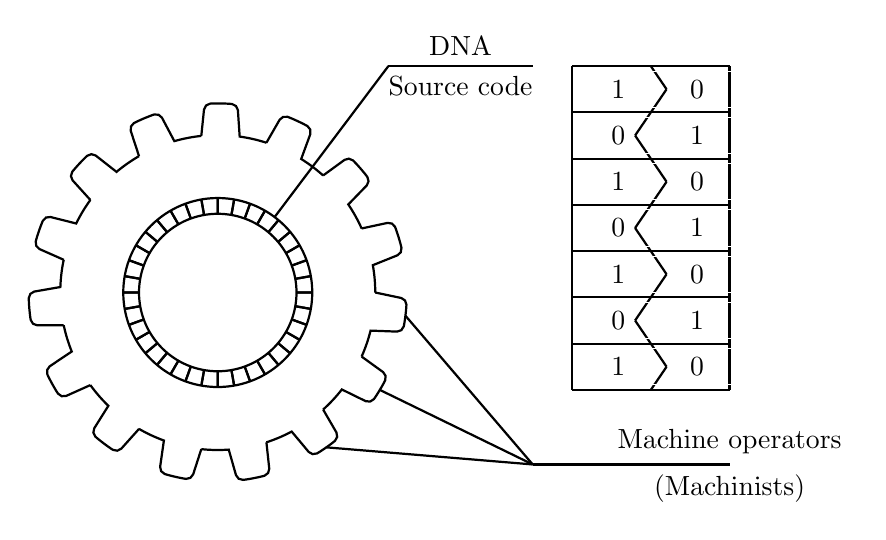
\begin{tikzpicture}
   \draw[thick] \gear{15}{2}{2.4}{10}{2}{1}{1.2}{0.0};

    \draw[thick,-] (0.7221780277824,0.9583626120564) -- (2.1665340833472,2.8750878361692); %53
    \draw[thick,-] (2.1665340833472,2.8750878361692) -- (4,2.8750878361692) node[midway,above]{DNA}node[midway,below]{Source code}; %53

    \draw[thick,-] (2.3821107639384,-0.292486424172) -- (4,-2.1835475811448); %-7
    \draw[thick,-] (2.0572015216848,-1.236091379784) -- (4,-2.1835475811448); %-31
    \draw[thick,-] (1.3765834472424,-1.9659649062936) -- (4,-2.1835475811448); %-55
    \draw[thick,-] (4,-2.1835475811448) -- (6.5,-2.1835475811448) node[right,below]{(Machinists)}node[right,above]{Machine operators};

    \draw[thick,-] (4.5,-1.236091379784) -- (4.5,2.8750878361692);
    \draw[thick,-] (6.5,-1.236091379784) -- (6.5,2.8750878361692);
    \draw[thick,-] (4.5,2.8750878361692) -- (6.5,2.8750878361692);
    \draw[thick,-] (4.5,-1.236091379784) -- (6.5,-1.236091379784);

    \draw[thick,-] (4.5,2.2877765196044574) -- (6.5,2.2877765196044574);
    \draw[thick,-] (4.5,1.7004652030397145) -- (6.5,1.7004652030397145);
    \draw[thick,-] (4.5,1.1131538864749716) -- (6.5,1.1131538864749716);
    \draw[thick,-] (4.5,0.5258425699102287) -- (6.5,0.5258425699102287);
    \draw[thick,-] (4.5,-0.0614687466545142) -- (6.5,-0.0614687466545142);
    \draw[thick,-] (4.5,-0.6487800632192571) -- (6.5,-0.6487800632192571);

    \draw[thick,-] (5.5,2.8750878361692) -- (5.7,2.58143217788682855);
    \draw[thick,-] (5.5,2.2877765196044574) -- (5.7,2.58143217788682855);

    \draw[thick,-] (5.5,2.2877765196044574) -- (5.3,1.99412086132208595);
    \draw[thick,-] (5.5,1.7004652030397145) -- (5.3,1.99412086132208595);

    \draw[thick,-] (5.5,1.7004652030397142) -- (5.7,1.40680954475734275);
    \draw[thick,-] (5.5,1.1131538864749713) -- (5.7,1.40680954475734275);

    \draw[thick,-] (5.5,1.1131538864749713) -- (5.3,0.81949822819259985);
    \draw[thick,-] (5.5,0.5258425699102287) -- (5.3,0.81949822819259985);

    \draw[thick,-] (5.5,0.5258425699102287) -- (5.7,0.23218691162785725);
    \draw[thick,-] (5.5,-0.0614687466545142) -- (5.7,0.23218691162785725);

    \draw[thick,-] (5.5,-0.0614687466545142) -- (5.3,-0.35512440493688565);
    \draw[thick,-] (5.5,-0.6487800632192571) -- (5.3,-0.35512440493688565);

    \draw[thick,-] (5.5,-0.6487800632192571) -- (5.7,-0.94243572150162855);
    \draw[thick,-] (5.5,-1.236091379784) -- (5.7,-0.94243572150162855);

    \node[draw,text width=2cm,draw=white] at (6,2.58143217788682855) {1};
    \node[draw,text width=2cm,draw=white] at (7,2.58143217788682855) {0};
    \node[draw,text width=2cm,draw=white] at (6,1.99412086132208595) {0};
    \node[draw,text width=2cm,draw=white] at (7,1.99412086132208595) {1};
    \node[draw,text width=2cm,draw=white] at (6,1.40680954475734275) {1};
    \node[draw,text width=2cm,draw=white] at (7,1.40680954475734275) {0};
    \node[draw,text width=2cm,draw=white] at (6,0.81949822819259985) {0};
    \node[draw,text width=2cm,draw=white] at (7,0.81949822819259985) {1};
    \node[draw,text width=2cm,draw=white] at (6,0.23218691162785725) {1};
    \node[draw,text width=2cm,draw=white] at (7,0.23218691162785725) {0};
    \node[draw,text width=2cm,draw=white] at (6,-0.35512440493688565) {0};
    \node[draw,text width=2cm,draw=white] at (7,-0.35512440493688565) {1};
    \node[draw,text width=2cm,draw=white] at (6,-0.94243572150162855) {1};
    \node[draw,text width=2cm,draw=white] at (7,-0.94243572150162855) {0};

\draw[thick]
\foreach \i in {1,2,...,36} {%
  [rotate=(\i-1)*10]  (0.0,1.0) -- (0.0,1.2)
};

 \end{tikzpicture}

}

\subsubsection{DNA}
\frame
{
The DNA is our central information storage of the complete ecosphere of  \texttt{The Machine}. Instead of four nucleobases like this is well known for example for human DNA we just use two which we have defined to be $$1$$ and $$0.$$As because classical computers also use such a binary storage model any kind of data that is stored inside a DNA can easily be copied on any classical computer or the other way round.
}

\subsubsection{Machine operator(s)}
\frame
{
\texttt{The Machine} operators are those who make a blanket rotate or work. They are also able to convert the blanket into a special gear just by changing their actions.
\newline
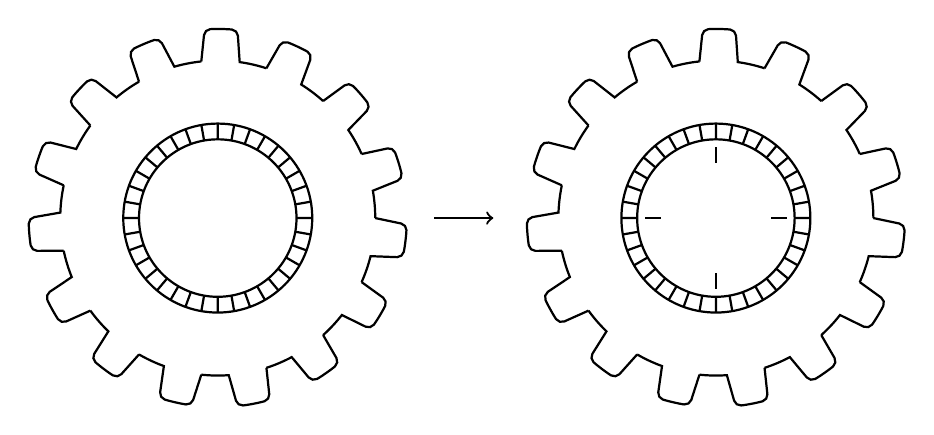
\begin{tikzpicture}
   \draw[thick] \gear{15}{2}{2.4}{10}{2}{1}{1.2}{0.0};
   \draw[thick, xshift=180] \gear{15}{2}{2.4}{10}{2}{1}{1.2}{180.0};
\draw[thick, xshift=180]
\foreach \i in {1,2,...,4} {%
  [rotate=(\i-1)*90]  (0.0,0.7) -- (0.0,0.9)
};
   \draw[thick,->] (2.75,0) -- (3.5,0);
 \end{tikzpicture}
}

\subsection{A Gear}
\frame
{

}

\section{The Machine}
\frame
{

}

\section{Summary}
\frame
{
%\frametitle{Summary}
\begin{itemize}
\item{\texttt{The Machine} is a complete self-contained cryptographic ecosphere driven by nothing but the Machinecoin cryptocurrency which is completely able to substitute any other well known classical (crypto)currency\footnote{machinecoin.org/wp-content/uploads/2014/04/value.pdf}.}
\item{Everybody can instantly and by themself become a new machinist and through this form his own blanket either alone or together with some friends and take part in the global \texttt{The Machine} movement.}
\item{Those who want to actively take part in the further development of \texttt{The Machine} movement can become a special gear inside of the community and help to make it even more better with every new day.}
\end{itemize}
}
\frame
{
%\frametitle{Summary}
Get started with the Machinecoin and join the global \texttt{The Machine} movement. All you need to do this is: you. Just either compile the given source code located at GitHub\footnote{github.com/gitju/machinecoin} or grab one of the already pre-compiled packages from the official Machinecoin website or any other Machinecoin Community Website\footnote{machinecoin.org (.de, .tk, .in, .tk, .eu, ...)} and configure it accordingly to your needs. You may also can get started just by using the Machinecoin Paper Wallet\footnote{paper.machinecoin.org} which allows you to create your very own Machinecoin address just within a couple of seconds. 
}

%\section{Bibliography}
%\begin{frame}
%	\frametitle{Quellen}
%	\bibliographystyle{alpha}
%	\bibliography{literatur}		
%\end{frame} 

\end{document}
%%%%%%%%%%%%%%%%%%%%%%
%%%  Dokument Ende                           
%%%%%%%%%%%%%%%%%%%%%%